\section{Durchführung}
\label{sec:Durchführung}
\subsection{Eigenschaften der Probe}
Zu Beginn des Versuches wird der elektrische Widerstand der Probe gemessen. In diesem Fall entsprach die Probe 
einem Draht aus Silber. Diese Messung erfolgt durch ein Multimeter.
Zudem wird eine Leiterplatte aus dem selben Material mittels einer Mikrometerschraube vermessen.
\subsection{Messung des Magnetfeldes}
Nun erfolgt die Messung eines Magnetfeldes, welches durch zwei Elektromagneten erzeugt wird. Zur Messung des 
Magnetfeldes wird eine Hallsonde zwischen die beiden Eisenkerne der Magnete gebracht. Dann wird die Stromstärke der
Spannungsquelle, die die Elektromagneten betreibt, von $\SI{0}{\ampere}$ in $\SI{0.5}{\ampere}$
Schritten bis $\SI{5}{\ampere}$ verändert. Dabei wird die von der Hallsonde gemessene magnetische Flussdichte
notiert. Die gleiche Messung wird erneut für ein umgepoltes Magnetfeld vorgenommen.
\subsection{Messung der Hallspannung}
Die Leiterplatte wird nun mit einer Spannungsquelle verbunden. Zudem wird sie 
senkrecht zu dem Magnetfeld in dieses eingehangen. Die Leiterplatte wird nun sowohl von einem Magnetfeld
als auch von einem elektrischen Strom durchflossen. Zur Messung der Hallspannung wird noch ein 
digitales Voltmeter an die Probe angeschlossen. Der beschriebene Versuchsaufbau ist in Abbildung
\ref{fig:versuchsanordnung} dargestellt.\\
%%Bild einfügen 
%
\begin{figure}[H]
    \centering
    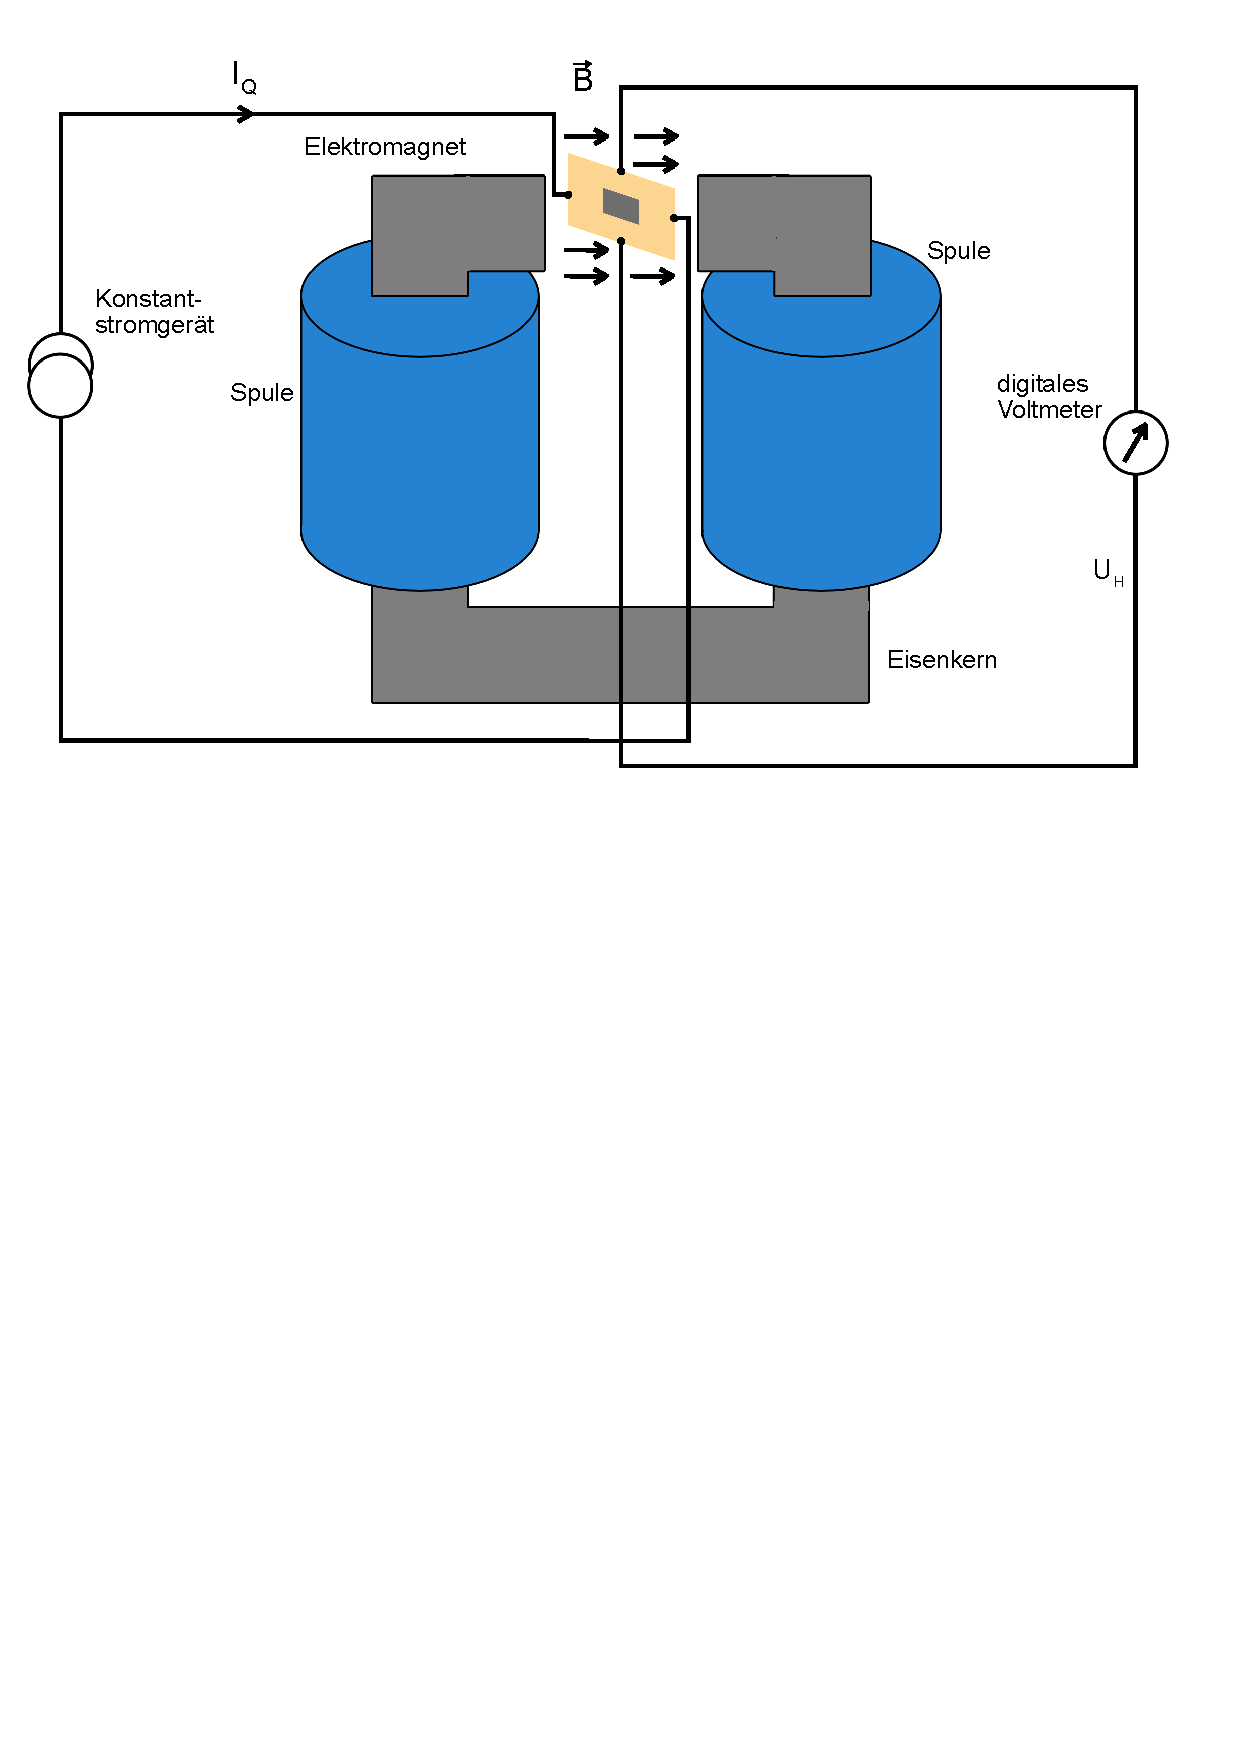
\includegraphics[scale = 0.3]{content/1Versuchsaufbau.pdf}
    \caption{Schematische Darstellung des Versuchsaufbaus}
    \label{fig:versuchsanordnung}
\end{figure}
%
Es werden nun zwei Messreihen durchgeführt:
\begin{enumerate}
    \item \textit{Messung bei konstantem Strom und variablem Magnetfeld}\\
        Die Spannungsquelle an der Leiterplatte liefert während dieser Messung einen konstanten Strom. 
        Verändert wird nur der Strom, welcher die Elektromagneten betreibt, wodurch sich die Intensität
        des Magnetfeldes ändert. Die Stromstärke wird dabei von $\SI{0}{\ampere}$ in $\SI{0.5}{\ampere}$
        Schritten bis $\SI{5}{\ampere}$ verändert. Nach jeder Veränderung des Magnetfeldes wird die 
        Hallspannung an dem digitalem Voltmeter abgelesen und notiert.\\
    \item \textit{Messung bei konstantem Magnetfeld und variablem Strom}\\
        Die Spannungsquelle an den Elektromagneten liefert während dieser Messung einen konstanten Strom und 
        somit ein konstantes Magnetfeld. 
        Verändert wird nur der Strom, welcher die Leiterplatte durchfließt.
        Die Stromstärke wird dabei von $\SI{0}{\ampere}$ in $\SI{0.5}{\ampere}$
        Schritten bis $\SI{5}{\ampere}$ verändert. Die Hallspannung wird wieder nach jeder Veränderung
        notiert.\\
\end{enumerate}
Beide Messreihen werden nun mit einem umgepolten Magnetfeld wiederholt.